\section{Introducción}
El trabajo expuesto en este documento tiene como fin la implantación de un museo virtual en el Observatorio de Madrid. La parte más importante en este tipo de proyectos (y, por extensión, de todos) es la recogida de requisitos y el análisis (en este caso, elección principalmente).
Para poder entender mejor lo que se solicita por parte del cliente es necesario conocer el concepto de "museo virtual" al que tratamos de acercarnos. Se trataría de una plataforma accesible físicamente desde puestos instalados en una sala de exposiciones dentro del propio observatorio, accesible en línea desde Internet y que comprenda una base de datos posiblemente reutilizable en el futuro. Con estas pinceladas he deducido que la solución existente (no hay que olvidar que esto es ingeniería) más cercana a lo que se nos pide pasaría, en mi opinión, por un gestor de contenidos o CMS (Content Management System).
Dada la amplísima oferta que hay de estos productos en el mercado, creo conveniente hacer una selección a partir de criterios, unos surgidos y otros sugeridos, analizados mano a mano con el cliente.
A partir de ahí, se escogerá el CMS candidato con mejores cualidades en cuanto a facilidad de uso, bajo mantenimiento y características incluidas por defecto. Las características no comprendidas en esta selección (pero necesarias igualmente) serán incorporadas junto con las diferentes modificaciones previstas para darle forma final a la plataforma. Posteriormente, se integrará y se pondrá en servicio con los plazos que el cliente disponga para ello.

\section{Base teórica}
Al tratarse de un proyecto tan práctico, la base teórica del mismo no tiene un gran misterio. Se trata de realizar el clásico enfoque de presentar distintas aplicaciones al cliente cumpliendo unos requerimientos mínimos y adpatanto e integrando la solución escogida para que encaje con el sistema solicitado.

En esta ocasión, presentaremos varios subapartados según las distintas fases del proyecto.

\subsection{Estado del Arte}
\par Para elaborar este proyecto pensé que lo más sensato era, una vez acotado el problema, tratar de echar un vistazo a cómo estaban las cosas en la actualidad en otros museos. Considero importante saber en qué estado se encuentran tanto el círculo de los CMS, wikis, museos y catálogos informatizados.
En este periplo, he topado con varias fuentes de información desconocidas para mí, algunas ideas sacadas de museos visitados en persona y una exhaustiva (aunque difícil de discernir) cantidad de datos sobre gestores de contenido.

\subsubsection{¿Qué puede ser un museo virtual?}
\par Al hablar de museos virtuales, a uno se le pueden venir a la mente distintos conceptos sobre lo que representan esas palabras:

\begin{itemize}
\item Visita virtual al museo (modo "Second Life").
\item Galería de imágenes.
\item Sitio web del museo (meramente informativo).
\item Catálogo de objetos.
\item Ampliación de lo expuesto en el museo.
\end{itemize}

\par En el primer caso, nos referimos a esa idea de recrear a través de gráficos en 3D la experiencia de una visita real al museo. Esta solución es muy poco usada debido a lo costoso de la misma. Además de modelar infográficamente la arquitectura del museo y construir una aplicación que utilice un potente motor gráfico para sostenerla, hay que tener en cuenta el gran tráfico generado para que esto funcione adecuadamente. En mi opinión, dado que difícilmente se puede reemplazar la experiencia de visitar el museo en persona, creo que no compensa tanto despliegue de medios ya que no contribuye (al menos en el caso expuesto) sensiblemente al objetivo marcado.

\par El segundo caso, una mera galería de imágenes, aunque pobre, podría vale como museo virtual para un museo de arte en según qué circunstancias. Obviamente, y aunque la presentación de la información en este formato sea algo a tener en cuenta, si limitáramos nuestro museo virtual a este tipo de sitio, estaríamos, creo yo, limitando muchísimo la información ofrecida, cosa que no cuadra con el objetivo de complementar el museo.

\par El tercer caso lo he incluído como posibilidad de que alguien lo identificase al hablar de "museos virtuales", dado que crear una página con información corporativa, de horarios y accesos es sólo una parte de lo que pretendería este proyecto.

\par El cuarto caso será aquel en el que básicamente tenemos una somera base de datos con una sencilla interfaz de búsqueda y acceso a la colección, sin tratar de explicar o poner en contexto los objetos que tenemos delante.

\par El quinto caso es el que nos ocupa, siendo el cometido del mismo complementar la exposición física, permitiendo a los visitantes (y no visitantes) conseguir un trasfondo y una explicación más completa de los objetos y su contexto para contribuir a la divulgación de un conocimiento relacionado con lo expuesto. Obviamente incluirá parte de galería de imágenes en cuanto a interfaz, información de típico sitio web como caso anecdótico de contenido, componentes que mejoren la interactividad sin sacrificar el desempeño y el coste y datos concretos sobre los objetos como manera de acceder a la base de datos. 

\subsubsection{Museos}

\par Aprendiendo de museos conocidos, podemos poner ejemplos prácticos de los que sacar ideas o matices que el cliente pueda identificar como deseables. Está claro que sería imposible abarcar todos o siquiera la mayoría de los museos del mundo, ni siquiera los más importantes (¿quién decide esa lista?), pero sin embargo sí se pueden incluir ideas que hayamos rescatado de otras implementaciones satisfactorias.
Algunos ejemplos son:

\paragraph{Tate Modern (Londres, Reino Unido)}
\par Pude comprobar en directo algunas de las ideas puestas en práctica por esta entidad gracias a un viaje reciente. Allí pude ver buenas ideas como el acercamiento de los contenidos de las salas al gran público (en especial, a niños) a base de actividades interactivas que introducían con naturalidad y entretenimiento conceptos difíciles de asimilar de otra manera. Sin duda es una buena idea, aunque no se encuadra en este proyecto, podría ser considerada para futuros trabajos. 
\par Más concretamente, en materia de museos virtuales, vi la adopción de terminales de mano que complementan la experiencia del visitante físico. Estamos acostumbrados a ver las típicas guías locutadas en diversos idiomas que nos amplían el contenido de las exposiciones introduciendo un número del índice de grabaciones. Suelen ser aparatos con usos muy restringidos (especiales para museos) con lo que eso supone para el coste final para el museo. En cambio, en este caso, se trataba de dispositivos móviles que están en el mercado, en nuestro caso, una especie de PDA de marca Toshiba o Dell (según renovaciones). Son dispositivos básicos que permiten mostrar contenidos web y multimedia sin muchas complicaciones. Esto es: pantalla en color, interfaz intuitiva, salida de auriculares y conectividad inalámbrica. Este último punto permite renovar sin coste temporal importante (y de manera transparente al visitante) los contenidos presentados. El hecho de que sea un dispositivo común abarataría los costes, premitiendo, incluso, trabajar con tecnología no necesariamente de última generación, dada la baja exigencia de los contenidos a presentar. Parece evidente que será más fácil conseguir un buen precio por una buena cantidad de dispositivos a punto de ser retirados del mercado o símplemente de stock sobrante.
Debajo de todo esto subyace la idea de utilizar unos estándares mínimos, aunque sean estándares de facto. Esto nos permitiría (como en el caso del Tate Modern) reemplazar los dispositivos por otros nuevos sin hacer cambios significativos en la plataforma y haciendo que coexistiesen ambos modelos. Y lo que es, quizá, más interesante, dar la opción a usuarios que posean dispositivos con capacidades similares a los ofrecidos de conectarse al museo virtual por su cuenta y en directo, ahorrando bastante en costes.

\paragraph{MoMA (New York, EEUU)}
\par Este apartado, desgraciadamente, se refiere a las ideas y modelos observados directamente en su página web. Nos encontramos con ideas, sobre todo en cuanto a presentación visual de contenidos. Digamos que la idea de presentar los contenidos en una matriz de imágenes con pies identificativos que, al pulsar sobre ellas, nos lleven a la información específica de ese objeto podría ser cercana a lo buscado. También sería una idea a tener en cuenta la categorización de las obras por área temática, época o tipo de objeto, aunque no lo firmamos como algo seguro en nuestra plataforma. Por último, reseñar que ellos parece que hacen (o al menos tienen la posibilidad de hacer) uso de la vista "por perspectivas". Esto sería como tener una lista desplegable en la pantalla que nos permitiera fácilmente cambiar entre los distintos puntos de vista (como si de idiomas se tratara) pudiendo adaptar la plataforma a una presentación para , por ejemplo, niños, estudiantes o expertos en el tema. El sistema finalmente escogido para implementar esa "granularidad" de contenidos se tomó de otro sitio web que veremos más adelante.


\paragraph{Actual museo del OAN}
\par Existe una versión antigua del museo virtual del Observatorio Astronómico Nacional, cuya información será contenida presumiblemente cuando se complete el contenido de la plataforma objeto de este proyecto. Si entramos al sitio web que lo hospeda dentro del sitio del Instituto Geográfico Nacional (Ministerio de fomento) descubrimos una estructura de navegación con algunas deficiencias para movernos entre objetos, para dar un vistazo rápido y desde luego una descontextualización importante. Podríamos catalogarlo como uno de esos museos virtuales del caso cuarto, un catálogo de objetos. No se puede negar su utilidad pero son las funciones de las que carece las que hacen necesaria la creación del proyecto actual.

\subsubsection{Enciclopedias}

\par Como parte de la gestión del conocimiento, además de las webs de los propios museos, he indagado en otras webs que se dedican a funciones parecidas (no olvidemos que el museo al que se refiere este trabajo dista de ser un museo de arte) a lo que queremos conseguir en cuanto a organización del conocimiento.

\paragraph{Wikipedia}
\par Digamos que este sería el paradigma de enciclopedia dinámica y colaborativa hoy en día. Es más o menos familiar para cualquier persona que use con asiduidad internet (sobre todo para buscar información) y aunque sus fuentes, consistencia y fiabilidad puedan ser cuestionables, su manera de disponer la información no puede tomarse en absoluto como mala. De aquí podríamos tomar en consideración el aspecto colaborativo del medio, pero en reuniones con el cliente se convino que al ser una institución de referencia, los contenidos (aunque aportados por diferentes personas) debían ser acotados a unos poco usuarios (generalmente trabajadores) y moderados en última instancia por la figura de un editor que revisaría y daría el visto bueno a los mismos.
La disposición de portal inicial ofrecida por este sitio es una idea que podría funcionar en nuestro caso, incluyendo esos pequeños "ganchos" que cambian diaria o aleatoriamente para que determinados artículos puedan ser descubiertos por un navegante no asiduo. Además, mantiene una división temática necesaria para el sitio y tiene un sistema de control de versiones válido para documentos escritos, así como la relación semántica de entradas y la inclusión de contenido multimedia fácilmente.
Referido al punto anterior, hay que señalar que, en un principio, se ha optado por la manera de Wikipedia de ampliar la profundidad de un artículo: en vez de diseñar distintas capas para distintos individuos, enlazar los artículos que profundizan sobre un tema para que sea el usuario el que decida cuándo parar.


\paragraph{Indianopedia, Frikipedia, *pedia}
\par Esta entrada engloba varios sitios por una razón: existe un fenómeno creciente que consiste en que cada "ecosistema" de conocimiento puede generar su propio repositorio de información. Esto contribuye a diversificar las fuentes evitando fraudes y manipulaciones, a la vez que descentraliza y permite pluralidad de visiones. Igual que existen el diccionario de la RAE, María Moliner, Espasa Calpe, etc., el concepto de la propia enciclopedia, en nuestro caso, puede servir para contener los artículos a los que no llegan otras enciclopedias más generales o de los que tenemos un conocimiento certero y fuentes propias.

\subsubsection{Sistemas gestores de contenidos vs Wikis}
\par Llegados a este punto parece evidente el camino que estamos sugiriendo. Para crear nuestra plataforma y que tenga algunos factores básicos como diferentes presentaciones al usuario (al menos internet y móviles), incluya una base de datos, interfaz amigable para creadores de contenido no informáticos y demás funciones de administrador facilitadas al máximo.

En un principio se tuvo la tentación de basar toda la plataforma en un mero wiki (La base de datos más simple del mundo) pero se vio que las características más destacables de un wiki nos sobraban salvo la facilidad de edición y de uso, que se puede apreciar también en los CMS más comunes. Además, claro está, si nos ciñéramos a un simple wiki estaríamos renunciando a una serie de herramientas útiles que ya se integran en los CMS con naturalidad.

De la toma de decisiones sobre la elección de plataforma base hablaré en la sección de diseño.


\section{Descripción del diseño}

\subsection{Baremación de alternativas}
\par Llegados a este punto, nuestro proyecto tiene que empezar a definirse y descartar unas alternativas de otras. Hasta la fecha, recapitulando, hemos puesto encima de la mesa la necesidad de un gestor de contenidos con o sin componente wiki. A este esqueleto inicial habría que añadirle una serie de características y su grado de importancia (donde 0 es prescindible y 5 es imprescindible). Este grado de importancia ha sido recogido en entrevista directa con responsables de la supervisión del proyecto.

\subsubsection{Relación de características}

\begin{tabular}{l @{\hspace{10px}} r}
Caracerística & Nota \\
\hline \\
Interfaz de creador en español & 4 \\
Interfaz de usuario en múltiples idiomas & 5 \\	
Varias perspectivas diferenciadas & 1 \\
Web semántica & 0 \\
Uso de estándares & 0 \\
Editor WYSIWYG & 5 \\
Soporte comercial & 1 \\
Comunidad de desarrolladores / soporte & 4 \\
Actualizaciones recientes & 1 \\
Entorno colaborativo & 3 \\
Buzón de sugerencia / Preguntas frecuentes & 0 \\
Página de control de cambios / CVS & 5 \\
Licencia libre & 5 \\
Base de datos & 3 \\
Sistema de ficheros (en contraposición a BD) & 0 \\
Posibilidad de exportar a pdf/LaTeX & 1 \\
Versión para plataformas móviles & 4 \\
Blog & 0 \\
\end{tabular}

\subsubsection{Comentarios}

\par La cuestión sobre las perspectivas diferenciadas se ha decidido plantear a la manera de Wikipedia, es decir, a base de enlaces con contenido más exhaustivo en vez de un selector de perspectiva que nos dejase "ponernos las gafas" de "estudiante", "visitante" o "investigador" con un botón, al menos, en esta fase del proyecto.

\par Aun no habiendo resuelto temas importantes como si la figura del "responsable de mantenimiento" de la aplicación existirá y quién se encargaría de ella, en la misma reunión se esbozó la idea de que existiría una fase inicial de carga con un principio y un final y una fase de mantenimiento en la que se harán cambios pero a menor ritmo. Todas ellas irán recubiertas de la figura del supervisor, que se encargará de aprobar o rechazar los cambios u añadidos propuestos por los generadores de contenido antes de que éstos se reflejen en la producción final.

\par En contrapartida a las ideas de blog y buzón de sugerencias, se propondrá (con mayor o menor grado de insistencia) al usuario realizar una encuesta evaluación con su propio espacio para sugerencias.

\par El tema de uso de estándares y web semántica, si bien es un objetivo deseable, no debe obstaculizar el resto de ellos, se asume de la última reunión.

\par Por último, y para que la base de datos creada pueda ser fácilmente usada por otros proyectos, se ha optado por buscar una solución orientada a bases de datos y no a sistemas de ficheros como modo de almacenamiento. Esto descartará unas cuantas opciones.

\subsection{Comparativa}

\par Habiendo descartado o relativizado la importancia de algunos de los requerimientos iniciales para nuestro gestor de contenidos, vamos a tratar de hacer una propuesta inicial. Para ello, vamos a utilizar herramientas gratuitas en línea que presentan los datos como una matriz de características (CMSMatrix.org y CMSMatch.com).

\subsubsection{Premisas iniciales}
\par Las premisas iniciales para los CMS (y las que más descartan) son:

\begin{itemize}
\item Más populares y mejor puntuados. De esta manera potencialmente hayaremos estabilidad y una comunidad de soporte activa. Para ello, echaremos un vistazo a las estadísticas disponibles en la red sobre CMS más utilzados, mejor puntuados y más premiados, tratando de sopesar adecuadamente cada fuente.
\item Editor visual (WYSIWYG Editor / Drag'n'Drop interface).
\item Con capacidad para gestionar la plataforma en varios idomas (Internationalization = Multilingual Content / Multilingual Content Integration / Web-based Translation Management).
\item Página de cambios (Versioning / Asset Management=Media Library)
\item Coste cero.
\item Licencia OpenSource.
\item Comunidad de desarrolladores (Developer Community).
\item Interfaz en español (Interface Localization).
\item Versión para móviles (Mobile Internet).
\end{itemize}

\subsubsection{Candidatos pre-seleccionados}
\par Primeros elegidos por su demostrada utilización, premios, etc:

\begin{enumerate}
\item dotCMS
\item Drupal
\item Joomla!
\item LifeRay Portal
\item MODx
\item mojoPortal
\item Moodle
\item Plone
\item SilverStripe
\item WordPress
\end{enumerate}

\par El primer problema que encontramos es que estos sistemas que hemos elegido para comparar los diferentes CMS no nos dejan saber qué idiomas tiene la interfaz de usuario, así que ha que hacer una pequeña investigación entrando en las páginas web de cada uno de los sitios. Tras esto, sabremos que, al menos en cuanto a la interfaz de administración, todas las plataformas preseleccionadas pueden ejecutarse en español.


\par A continuación, pasamos a desgranar las dos comparativas hechas con las diferentes herramientas encontradas:

\subsubsection{Comparativa con CMSMatrix}

\par En esta ocasión, vamos a ir comparando las características más reseñables de cada producto, por bloques, según está organizado en el servicio consultado.

\paragraph{System Requeriments (Requisitos de sistema)}

\par Vamos a ir analizando lo que se ve en la figura:

\begin{figure}
\begin{narrow}{-0.2\linewidth}{-0.2\linewidth}
\centering
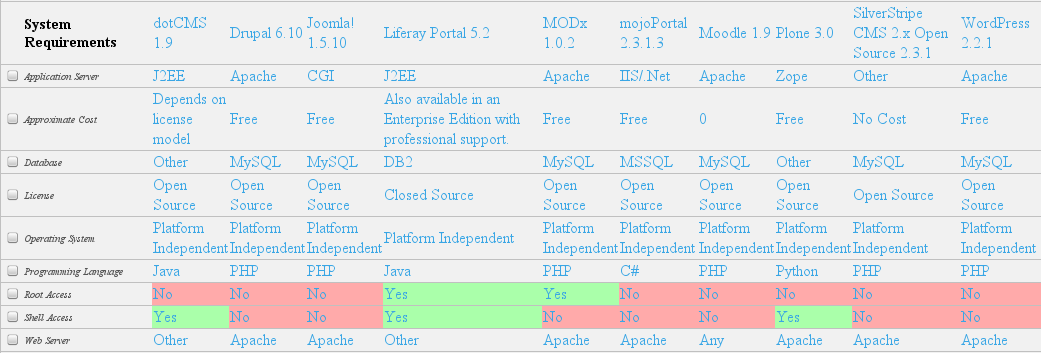
\includegraphics[width=\linewidth]{cmsmat1}
\caption{System Requeriments desde CMSMatrix.org}
\end{narrow}
\label{fig:cmsmat1}
\end{figure}

%\begin{sidewaysfigure}
%  \centering
%   \includegraphics[width=\textheight]{proyecto2}
%\caption{Diagrama de Gantt del proyecto}
%\label{fig:gantt2}
%\end{sidewaysfigure}


\section{Conclusiones y trabajo futuro}


